%%% This is the master's thesis for William Woodall
%%%  It is based on the Auburn Thesis template by Chris Wilson

%%%%%%%%%%%%%%%%%%%%%%%%%%%%%%%%%%%%%%%
%% Document Configuration
%%%%%%%%%%%%%%%%%%%%%%%%%%%%%%%%%%%%%%%

\documentclass[12pt]{report}
\usepackage{aums}        % For Master's papers
% \usepackage{auphd}       % For Ph.D.
% \usepackage{auhonors}    % For honors college
\usepackage{ulem}        % underlining on style-page; see \normalem below
\usepackage{url}
% \usepackage{tikz}
% \usepackage{pgf}
\usepackage{amsmath}
\usepackage{cite}
\usepackage{subfig}
% \usepackage{lineno}  % Inserts line numbers

%% For Algorithms
\usepackage{algorithm}
\usepackage{algorithmic}

%% For graphics
\usepackage[pdftex]{graphicx}
\graphicspath{{figures/}}
\DeclareGraphicsExtensions{.pdf,.jpeg,.png}

% adjust size of line numbers
% \def\linenumberfont{\normalfont\small\sffamily}

%%%%% Format rules: Normal margins are 1 in.
%%%%% If you need to print with 1.5in margins, uncomment the line below
% \oddsidemargin0.5in \textwidth6in

%% If you do not need a List of Abbreviations,
%% then comment out the lines below and the \printnomenclature line.
%% for List of Abbreviations information:
%%  (see http://www.Mackinac.com/TECHTALK/509.htm  )
\usepackage[intoc]{nomencl}
\renewcommand{\nomname}{List of Abbreviations}           
\makenomenclature 
%% don't forget to run:   makeindex ausample.nlo -s nomencl.ist -o ausample.nls

% May want theorems numbered by chapter
\newtheorem{theorem}{Theorem}[chapter]

%%%%%%%%%%%%%%%%%%%%%%%%%%%%%%%%%%%%%%%
%% Title Page Configuration
%%%%%%%%%%%%%%%%%%%%%%%%%%%%%%%%%%%%%%%

% Put the title, author, and date in. 
\title{3D Teleoperation with the Microsoft Kinect}
\author{William J. Woodall IV}
\date{August 4th, 2012} % date of graduation
\copyrightyear{2012} % copyright year

\keywords{teleoperation, mapping, robotics, octree, Kinect}

% Put the Thesis Adviser here.
\adviser{Sa\^{a}d Biaz}

% Put the committee here (including the adviser), one \professor for each. 
% The advisor must be first, and the dean of the graduate school must be last.
\professor{Sa\^{a}d Biaz, Chair, Associate Professor of Computer Science and Software Engineering}

\professor{David M. Bevly, Co-Chair, Albert Smith Jr. Professor of Mechanical Engineering}

\professor{John Y. Hung, Professor of Electrical and Computer Engineering}

\begin{document}

% \linenumbers  % turn on line numbers for editorial needs

\begin{romanpages}      % roman-numbered pages 

\TitlePage 

%%%%%%%%%%%%%%%%%%%%%%%%%%%%%%%%%%%%%%%
%% Abstract
%%%%%%%%%%%%%%%%%%%%%%%%%%%%%%%%%%%%%%%

\begin{abstract} 
This thesis investigates the feasibility of using novel three dimensional sensors like the Microsoft Kinect\cite{KINECT} and the Asus Xtion Pro Live\cite{ASUS} to assist the teleoperation of mobile vehicles.  Ultimately this work would be applicable to any teleoperated vehicle equipped with sensors providing three dimensional data of the environment, such as an automated ATV with a stereo vision system or a Velodyne LiDAR\cite{halterman2010velodyne} system.  The challenges related to utilizing dense three dimensional data in a way that is practical for teleoperation scenarios are identified and solutions are proposed and implemented.  To simplify the approach, the problem is split into three smaller tasks: three dimensional mapping, teleoperation and telemetry visualization, and latency reduction techniques.  The three dimensional mapping pertains to using the three dimensional sensor data in concert with the mobile vehicle navigation solution to generate a three dimensional map of the environment in real-time.  The resulting map must be efficiently sent to the teleoperator and visualized in the teleoperation and telemetry visualization section.  Additionally, latency greatly reduces the teleoperator's ability to drive the vehicle, so methods for reducing the perceived latency are investigated, including using a vehicle model to simulate the vehicle motion in the absence of timely telemetry updates.
\end{abstract}

%%%%%%%%%%%%%%%%%%%%%%%%%%%%%%%%%%%%%%%
%% Acknowledgments
%%%%%%%%%%%%%%%%%%%%%%%%%%%%%%%%%%%%%%%

\begin{acknowledgments}
Acknowledge people here.
% TODO: this
\end{acknowledgments}

\tableofcontents
\listoffigures
\listoftables
\listofalgorithms

\printnomenclature[0.5in] %used for the List of Abbreviations
\end{romanpages}        % All done with roman-numbered pages


\normalem       % Make italics the default for \em

%%%%%%%%%%%%%%%%%%%%%%%%%%%%%%%%%%%%%%%
%% Chapter: Introduction
%%%%%%%%%%%%%%%%%%%%%%%%%%%%%%%%%%%%%%%

\chapter{Introduction}\label{chap:introduction}
This work is motivated by the need for improved teleoperation techniques in commercial and military applications.  Given three dimensional information about the environment a much better representation of the environment can be presented to the teleoperator.  This provides an advantage to traditional two dimensional images by providing spatial awareness and multiple view points of the same scene.  Applications of this sort of technology include: maneuvering a teleoperated vehicle in tight quarters like a city alley, teleoperating a robotic arm in a cluttered environment, or navigating an indoor robot in an office environment.  The advantages of this three dimensional map bring related disadvantages that must be minimized in many teleoperation scenarios to make the benefit worth the cost.  In most teleoperation scenarios things like computing resources, battery life, power, and bandwidth are at a premium.  This is problematic when considering the three dimensional mapping system as it can use considerable computer resources to process the three dimensional data and produce a map of the environment.  Additionally, the resulting map can be quite large, depending on the resolution of the map and the size of the area being represented.  Thus, when considering the use of these three dimensional maps in teleoperation scenarios, techniques for minimizing the processing and bandwidth must be considered.  Furthermore, in many teleoperation scenarios the communications link is quite latent, due to being a satellite or cellular system.  The increased latency in a teleoperation system significantly reduces the teleoperator's ability to control the vehicle, impacting both their obstacle avoidance capabilities and top speeds\cite{photo_real}.

\section{Mapping}
Mapping three dimensional environments has become a hot research topic in the past few years, and some amount of that trend can be attributed to the Microsoft Kinect\cite{KINECT}.  Since its release in November of 2010\cite{GIZMODO}, the Kinect has enabled researchers and enthusiasts all over the world by giving them access to high quality three dimensional data in an available and affordable sensor package.  The experimental part of this work takes advantage of the innovation of Kinect technology and applies it to the teleoperation of mobile robot vehicles.

With the increasing availability of three dimensional spatial data from sensors like the Primesense based RGB-Depth cameras \cite{PRIMESENSE} and registering sweeping laser range finders with cameras \cite{photo_real}, being able to store, transmit and manipulate this data in an efficient manner has become important.  There are a number of applications for this type of 3D information, for example: 3D or 6D SLAM \cite{biswasdepth}, 3D teleoperation \cite{photo_real}, and robotic path planning \cite{3DCOLLISION}.  Because of this surge in the availability of three dimensional data, commonly represented as a point cloud, a new open library aimed at manipulating and processing point clouds has risen to popularity.  This library is known as the the Point Cloud Library (PCL)\cite{rusu20113d}, and it provides many high quality data structures and algorithms for processing points clouds.
  
Outdoor and Indoor environments can be difficult to capture in full three dimensional space. One of the issues with mapping three dimensional space is that the computing resources (like processing time, memory usage, and network bandwidth) can be prohibitive to storing, transmitting, and processing the map. Octrees have a long history of being used in 3D applications\cite{boada2001multiresolution}, surface reconstruction\cite{kazhdan2006poisson}, and computer graphics\cite{fang1996deformable}. Recent work has shown that three dimensional maps can be stored efficiently using octrees for use in robotics applications\cite{octomap}. The research by A. Hornung, et. al. resulted in an open source library called octomap \cite{octomap}. The primary use of the octomap library so far has been in occupancy based motion planning for robots and robotic manipulators \cite{3DCOLLISION}. This paper applies this octree based spatial database methods described in the octomap paper to mapping three dimensional environments with teleoperation of robotic vehicles in mind.

%% TODO: Add a section about teleoperation here to balance the mapping section.

The rest of this thesis will cover the system design process and resulting artifacts in Chapter \ref{chap:system_design}, the three dimensional mapping subsystem in Chapter \ref{chap:3d_mapping}, the teleoperation subsystem in Chapter \ref{chap:teleoperation}, discuss the techniques for latency reduction in Chapter \ref{chap:latency_reduction}, describe the experimental setup and results in Chapter \ref{chap:experiments}, and finally draw some conclusions and look toward future work in Chapter \ref{chap:conclusion}.

%%%%%%%%%%%%%%%%%%%%%%%%%%%%%%%%%%%%%%%
%% Chapter: System Design
%%%%%%%%%%%%%%%%%%%%%%%%%%%%%%%%%%%%%%%

\chapter{System Design}\label{chap:system_design}
Before jumping into the system design, previous work in related projects was surveyed.  This allows for a better perspective on the field before considering the scope and layout of the system.

There are several groups that have previously aimed to provide a more photo realistic three dimensional environment in order to improve teleoperation scenarios.  In particular Huber, et. al. from Carnegie Mellon University describe a system with a multi faceted approach to representing the environment in three dimensional space\cite{photo_real}.  Their system showed that it was possible to achieve a high level of fidelity when representing the environment.  They employed several techniques to reconstruct the environment including billboards, voxel grids, point clouds, and ground plane estimation and modeling.  Additionally, they showed that their system improved teleoperation of automated vehicles and they characterized the affects of latency on the teleoperators.  What their work did not address was the problems of processing or bandwidth.  Their system had an umbilical fiber optic cable to transmit the telemetry back to an on site trailer where the telemetry was converted into the three dimensional components using a rack of several servers.  Therefore, one of th goals of this thesis is to address some of those concerns by simplifying the representation of the three dimensional environment and by leveraging different storage structures and methodologies when building the map and transmitting it to the teleoperator.

\section{Problem Statement and Requirements Analysis}
The system should take telemetry from the robotic vehicle, and use it to produce a visually accurate three dimensional map of the vehicle's environment.  The resulting map should be displayed to the user, also known as the teleoperator, and the user's input should be used to control the robotic vehicle.  The robot's telemetry should include both proprioceptive data which will provide information about the location of the vehicle in its environment and exteroceptive data which provides three dimensional data about the environment.  By combining these two types of data a three dimensional model of the vehicle is placed in a reconstruction of the environment and is displayed to the teleoperator.  The mechanism by which the reconstructed environment is transmitted to the teleoperator must work in low bandwidth and high latency networks.

\subsection{System of Systems Architecture}
The system design follows from the problem statement and the requirements analysis as a system of systems in a client-server architecture.  The system can clearly be divided into a robotic vehicle subsystem, a three dimensional mapping subsystem, and a teleoperation subsystem.  The robotic vehicle subsystem can be abstracted and therefore decoupled from the mapping and teleoperation subsystems.  The three dimensional mapping system takes the abstracted telemetry from the robotic vehicle with which it maintains a three dimensional map of the environment.  This map is then provided to the teleoperation system which transmits the map and visualizes it for the teleoperator.  Additionally the teleoperation subsystem takes the user input which is communicated to the robotic vehicles abstracted command interface, again decoupling it from the other subsystems.  The teleoperator, and his machine, can be viewed as the client and the robotic vehicle is the server which provides processed telemetry and executes input from the teleoperator.  A high level diagram of the system is seen in figure \ref{fig:subsystem}.

\begin{figure}[ht]
  \centering
  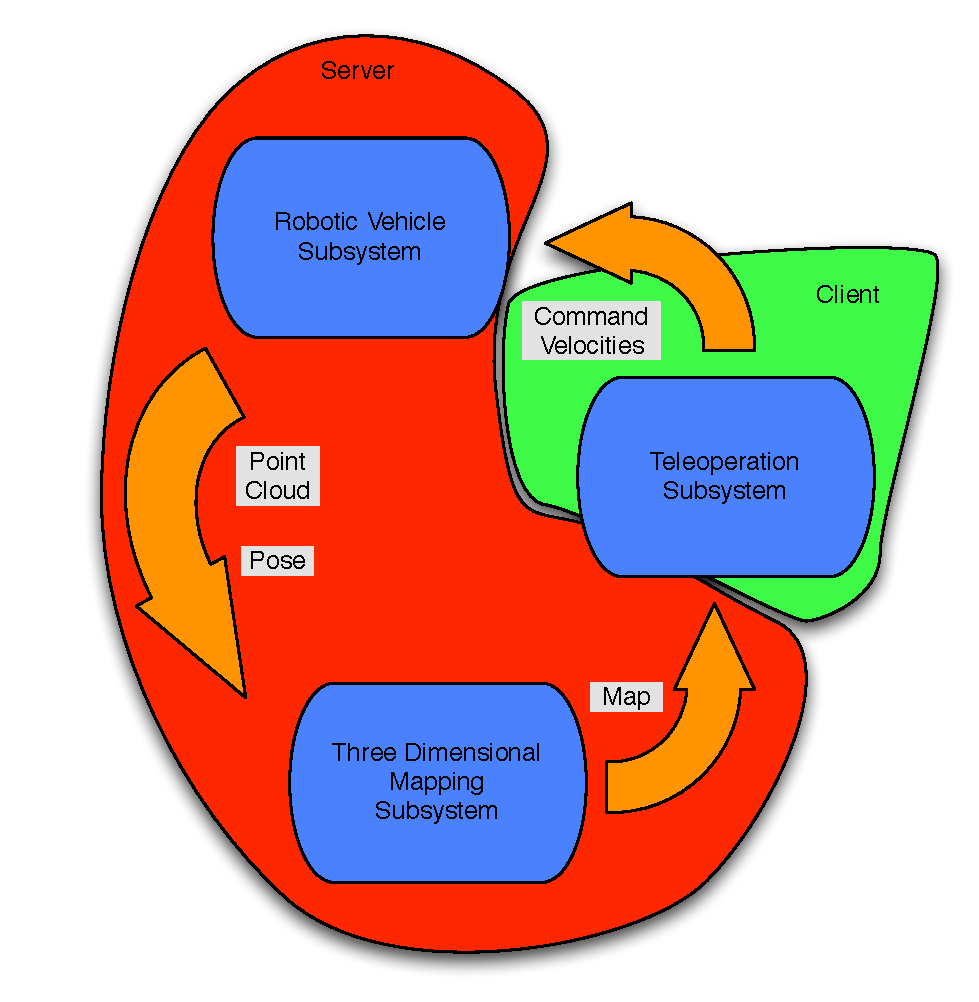
\includegraphics[width=5in,keepaspectratio]{subsystem.pdf}
  \caption{Subsystem Layout}
  \label{fig:subsystem}
\end{figure}

An assumption about the design is made in the above paragraph.  The assumption is that all of the telemetry is processed by the mapping subsystem before being transmitted by the teleoperation subsystem.  It would be possible to transmit the raw telemetry to the teleoperator and then processed on the teleoperator's machine.  The reason this was not the selected design pattern was because the network bandwidth and latency is at a higher premium than the processing power available on the robotic vehicle.  This design attempts to meet the lowest common denominator by minimizing processing for the mapping and then transmitting the completed map, which can be much more concise than the raw telemetry.

By decoupling the three subsystems, it makes replacing one implementation of a subsystem with another much easier.  Because the robotic vehicle's interfaces consist of one or more exteroceptive sensors, a proprioceptive pose solution, and a velocity command interface, the underlying robotic vehicle can be replaced with any robotic subsystem that can conform to that interface.  Similarly, the mapping subsystem can be replaced with any individual mapping system that takes the telemetry from the robotic vehicle and produces a map for the teleoperation subsystem.

\section{System Specification}
Breaking the subsystems down further, implementation specific details begin to come to light.  Figure \ref{fig:system_diagram} shows the three subsystems in more detail and more tightly integrated.  Thought the interfaces are missing here the flow of information remains the same from the subsystem layout in Figure \ref{fig:subsystem}.

\begin{figure}[ht]
  \centering
  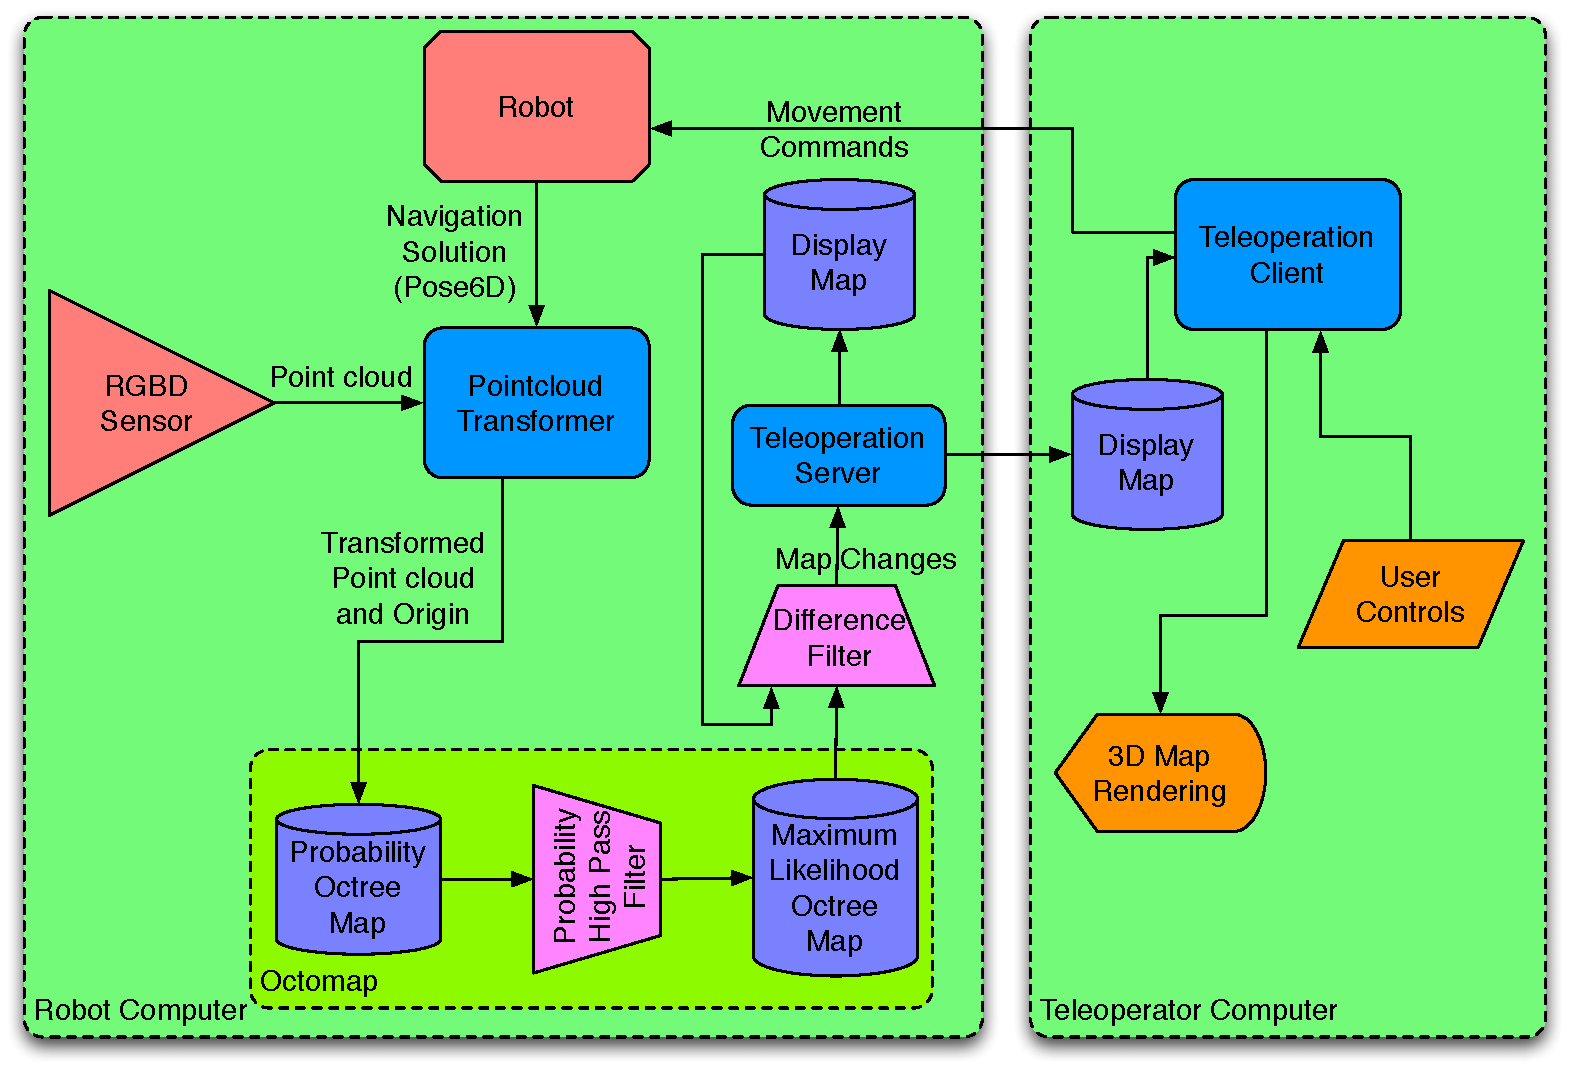
\includegraphics[width=6in,keepaspectratio]{system_diagram.pdf}
  \caption{System Design}
  \label{fig:system_diagram}
\end{figure}

As mentioned above Figure \ref{fig:system_diagram} describes the overall system design.  The three dimensional data in the form of point clouds are collected from one or more sensors, like the Microsoft Kinect.  These point clouds are combined with a navigation solution from the robotic base to transform the data points into a common map coordinate frame.  At this point the point clouds are inserted into the map using a probabilistic insertion method which is described in Chapter \ref{chap:3d_mapping}.  A maximum likelihood version of the map is generated and is stored in, what this work will refer to as, the server map.  At this point the map is ready to be used in teleoperation, so the server map is subtracted from the map that the client current has, referred to as the client map.  The differences, or part of the differences, are sent to the client and united with the current client map.  If all of the differences are sent, then the client map and the server map should then be synchronized, otherwise successive iterations of this process will eventually result in an up-to-date client map.  Simultaneously, input from the teleoperator is being sent to the robotic vehicle to allow teleoperation.

The above description, or theory of operation, of the system makes references to several, as yet, undefined processes and design decisions.  There are more details on the Mapping and Teleoperation subsystems in Chapters \ref{chap:3d_mapping} and \ref{chap:teleoperation}, respectively.  The robotic subsystem and it's fore mentioned navigation solution are discussed in the next section and the Experimental Setup in Section \ref{sec:experimental_setup}.

\section{Robot Navigation}
A necessary component of the proposed teleoperation system is the ability for the robotic vehicle to provide an accurate pose estimate.  Because the system proposed does not rely on ICP or feature mapping to combine successive point clouds, as in P. Henry, M. Krainin, and E. Herbst\cite{Henry2010}, the pose estimate from the robotic vehicle must be very accurate.  The trade off is that a much smaller amount of processing is required to generate the map, but the resulting quality of the map is sensitive to errors in the pose estimate.  Outdoor navigation systems like the Novatel SPAN system can provide \textasciitilde2 centimeters positional accuracy and 1/10th degree angular accuracy\cite{kennedy2006architecture}, which would be acceptable.  Indoor robots, like the experimental setup for this paper, require some other means of estimating its position in an arbitrary global coordinate frame.  The experimental system in this work uses an implementation of grid SLAM, which combines odometry from the wheel encoders with laser range finder data from a Sick LMS151.  An off-the-shelf SLAM library is used to get a high quality pose estimate indoors, and it uses a grid based approach with particle filters to map and localize on the environment.  The library used is called the gmapping library\cite{grisetti2007improved}\cite{grisettiyz2005improving}, which is an open source library and can be found on openslam.org.  This gives a high accuracy, drift free pose solution of the vehicle indoors.

%%%%%%%%%%%%%%%%%%%%%%%%%%%%%%%%%%%%%%%
%% Chapter: Three Dimensional Mapping
%%%%%%%%%%%%%%%%%%%%%%%%%%%%%%%%%%%%%%%

\chapter{Three Dimensional Mapping}\label{chap:3d_mapping}
As with the top level system design, previous mapping solutions are analyzed before design begins.  In the following section a survey of past work is presented.

\section{Previous Work}
\label{sec:previouswork_3dmapping}
Recent work has been done to create three dimensional maps of the environment using octrees and a probabilistic insertion method that is well suited for robotic activities where there is noise in the data and uncertainty in the pose of the robot. A. Hornung, et. al. described and implemented this system and it resulted in an open-source library called octomap.\cite{octomap} This paper uses octomap as the octree mapping system and exactly how that works is described in section \ref{sec:3dmapping}.  There are two main elements of the octomap research that are useful in a three dimensional teleoperation system.

First, the probabilistic method for adding new three dimensional information to the map is ideal for a system that needs to be updated continuously.  Uncertainty from the navigation solution will result in point clouds that are transformed slightly incorrect, and this causes inconsistencies and skews in the resulting map. The probabilistic manner in which the scans are inserted into the octree help to alleviate this inconsistency by allowing for some error in the point clouds in relation to map. This is further alleviated by the nature of the octree data structure, because inserting the point clouds into the octree essentially results in a down sampling of the original data to the resolution of the octree.

Second, limiting the query depth on the octree will effectively and efficiently down sample the map.  This allows for an adjustable quality level of the map being sent over the wire to match the available resources like network bandwidth and network latency.  This is important because most teleoperation systems work over a wireless and unreliable communication layer, which often suffers from low data rates and large latencies.  An analogy can be drawn to how on-line video streaming services will adjust the compression of a video to accommodate the connection being used, but in these systems the main concern is bandwidth not latency.

In addition to the work done by A. Hornung, et. al. with octomap, three dimensional mapping done specifically with RGB-D camera's from Primesense was done by P. Henry, M. Krainin, and E. Herbst.\cite{Henry2010}  In this paper they used alignment techniques like features with RANSAC, ICP and loop closure techniques to produce a very high quality map from the RGB-D data.\cite{Henry2010}  This approach differs from this paper in that this system relies on other sensors and existing navigation solutions to provide accurate transforms for the points clouds in an attempt to make the system more processor efficient and run closer to real time.  The work by P. Henry, M. Krainin, and E. Herbst still managed to perform the processing in a relatively small amount of time, but at the publishing of that paper had not gotten it up to the speeds required for real time teleoperation.

Very recent work by Microsoft using the Kinect has achieved real-time mapping with the Kinect in a project called KinectFusion\cite{izadi2011kinectfusion}.  Additional work has seen this technology demo reproduced using PCL and extended spatially\cite{whelankintinuous}.  This technique employs new methods for combining Kinect data on the Graphics Processing Unit of the computer's video card.  This technology is very young, but most likely will be a suitable replacement for the mapping system presented in this work.  The only benefit to the mapping system presented in this work is that it still requires far less processing than the KinectFusion system.

\section{The Mapping Process}
\label{sec:3dmapping}
This section describes the process of combining the three dimensional data from the sensor and six dimensional poses from the robot base into three dimensional maps of the environment. As previously mentioned in Section \ref{sec:previouswork_3dmapping}, A. Hornung, et. al. have already shown that octrees combined with a probabilistic insertion method can provide a good solution when creating three dimensional maps in this manner. A portion of this section is just explaining their work and how it is used in the teleoperation system described in this thesis work.\cite{octomap} The obvious first steps of this process is obtaining the three dimensional data and the six dimensional pose of the robotic base from which the map is constructed, but these are described briefly in Section \ref{sec:experimental_setup}.

\subsection{Transforming the Point Clouds}
Each time new data from the three dimensional sensor is received by the computer the data needs to be transformed into a common arbitrary global frame or `map' frame. Figure \ref{fig:transforms} shows a typical transformation tree for the robotic setup. The `base\textunderscore{}link' frame is commonly referred to as the vehicle frame. The transformation between the `map' frame and the `base\textunderscore{}link' frame represents absolute transformation given by robotic vehicle's pose estimate. The transformations between the `base\textunderscore{}link' frame and the `laser\textunderscore{}link' frame and the `camera\textunderscore{}link' frame are static geometric relationships and represent the position of the sensors on the robot chassis. When new point clouds are receive they are in the `camera\textunderscore{}link' coordinate frame and need to be converted into the `map' coordinate frame as that is the corrected global frame in this situation.

\begin{figure}[ht]
  \centering
  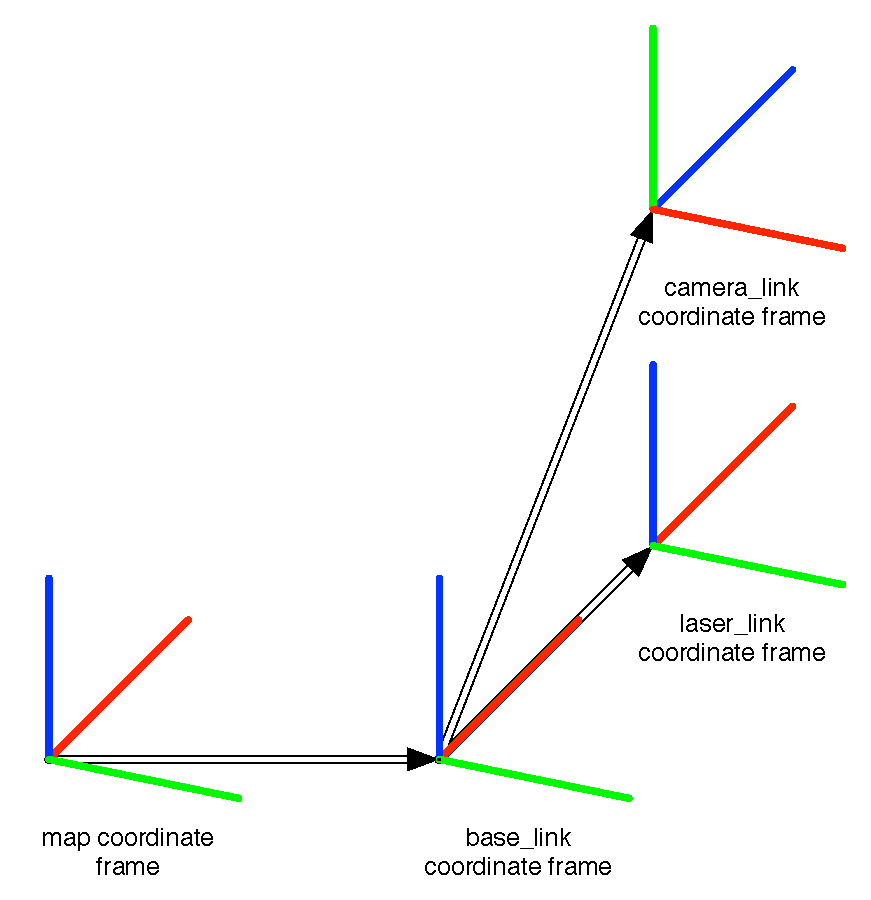
\includegraphics[width=5in,keepaspectratio]{transforms.pdf}
  \caption{Typical Coordinate Transform Tree}
  \label{fig:transforms}
\end{figure}

\subsection{Inserting New Data}
Once the point cloud data has been transformed into the global coordinate frame the data needs to be added to the map. As previously mentioned, this is done by the octomap library, but the process is described here for clarity. The underlying data structure for this map is an octree where each leaf has a probability of occupation. This in effect is a three dimensional occupancy grid with octree storage where each leaf of the tree is a voxel in the grid. The transformed data and the origin of the sensor in the global coordinate frame are required for the insertion. The insertion method starts by iteratively ray tracing from the origin of the sensor to each data point in the point cloud.  For each voxel that the ray trace passes through the probability of occupation of for that voxel is decreased by a given amount. For the voxel that the ray trace ends in the probability of that voxel being occupied is increased by a given amount. In this way it takes several points falling into a voxel to have voxel considered to be occupied and allows for fringe voxels caused by noise to be cleared by additional new data.

\begin{figure}[ht]
  \centering
  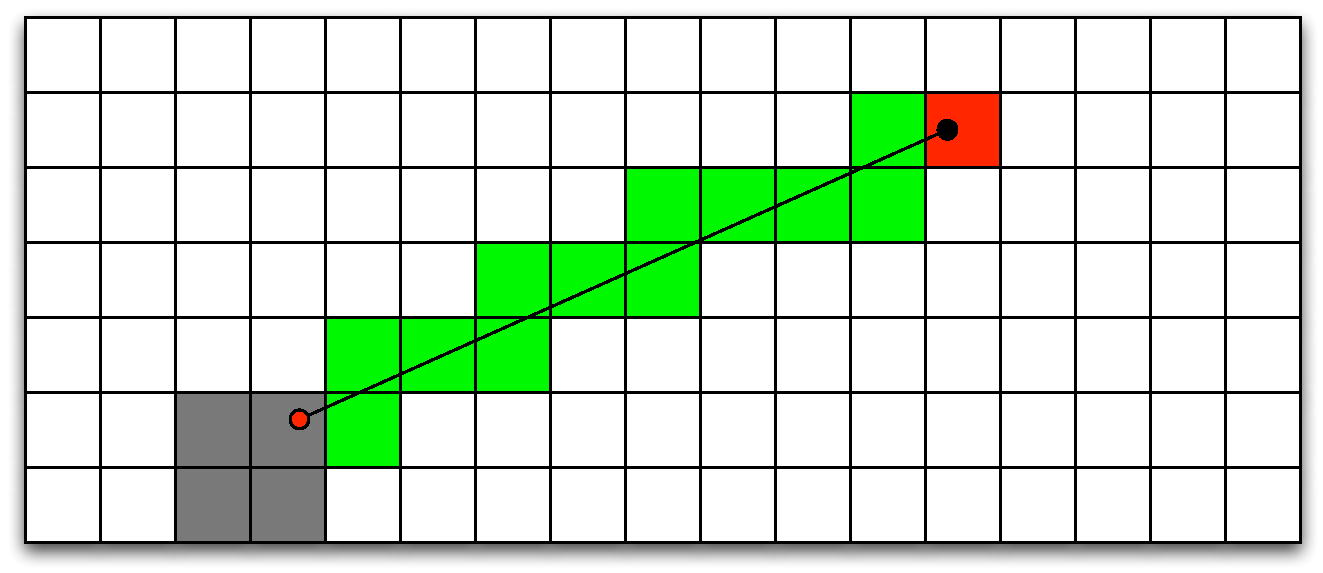
\includegraphics[width=5in,keepaspectratio]{raytrace.pdf}
  \caption{Two Dimensional Example of Voxel Raytracing.}
  \label{fig:voxel_raytrace}
\end{figure}

Figure \ref{fig:voxel_raytrace} shows this process in a two dimensional example where the gray voxels are the robot, the red dot is the sensor origin, the black dot is the point from the point cloud, the green voxels are having their occupancy decreased, and the red voxel is having its occupancy increased. This method of voxel ray tracing is originally proposed by Amanatides, J. and Woo, A., and is referenced in the octomap paper.\cite{amanatides1987fast}

\section{Sources of Error During Three Dimensional Mapping}
With this approach to three dimensional mapping, map quality can be adversely affected by several different sources of error, including the uncertainty in the pose estimate of the robotic vehicle, random and systematic error in the three dimensional data, and systematic errors due to timing and geometric misalignment.  Figure \ref{fig:slamvsoctree} shows the resulting octree map with the map from the Simultaneous Localization and Mapping (SLAM) algorithm, which is good enough in this instance to be considered truth. The octree map generally lines up with the SLAM map but has a lot of areas where the result is less than desirable.

\begin{figure}[ht]
  \centering
  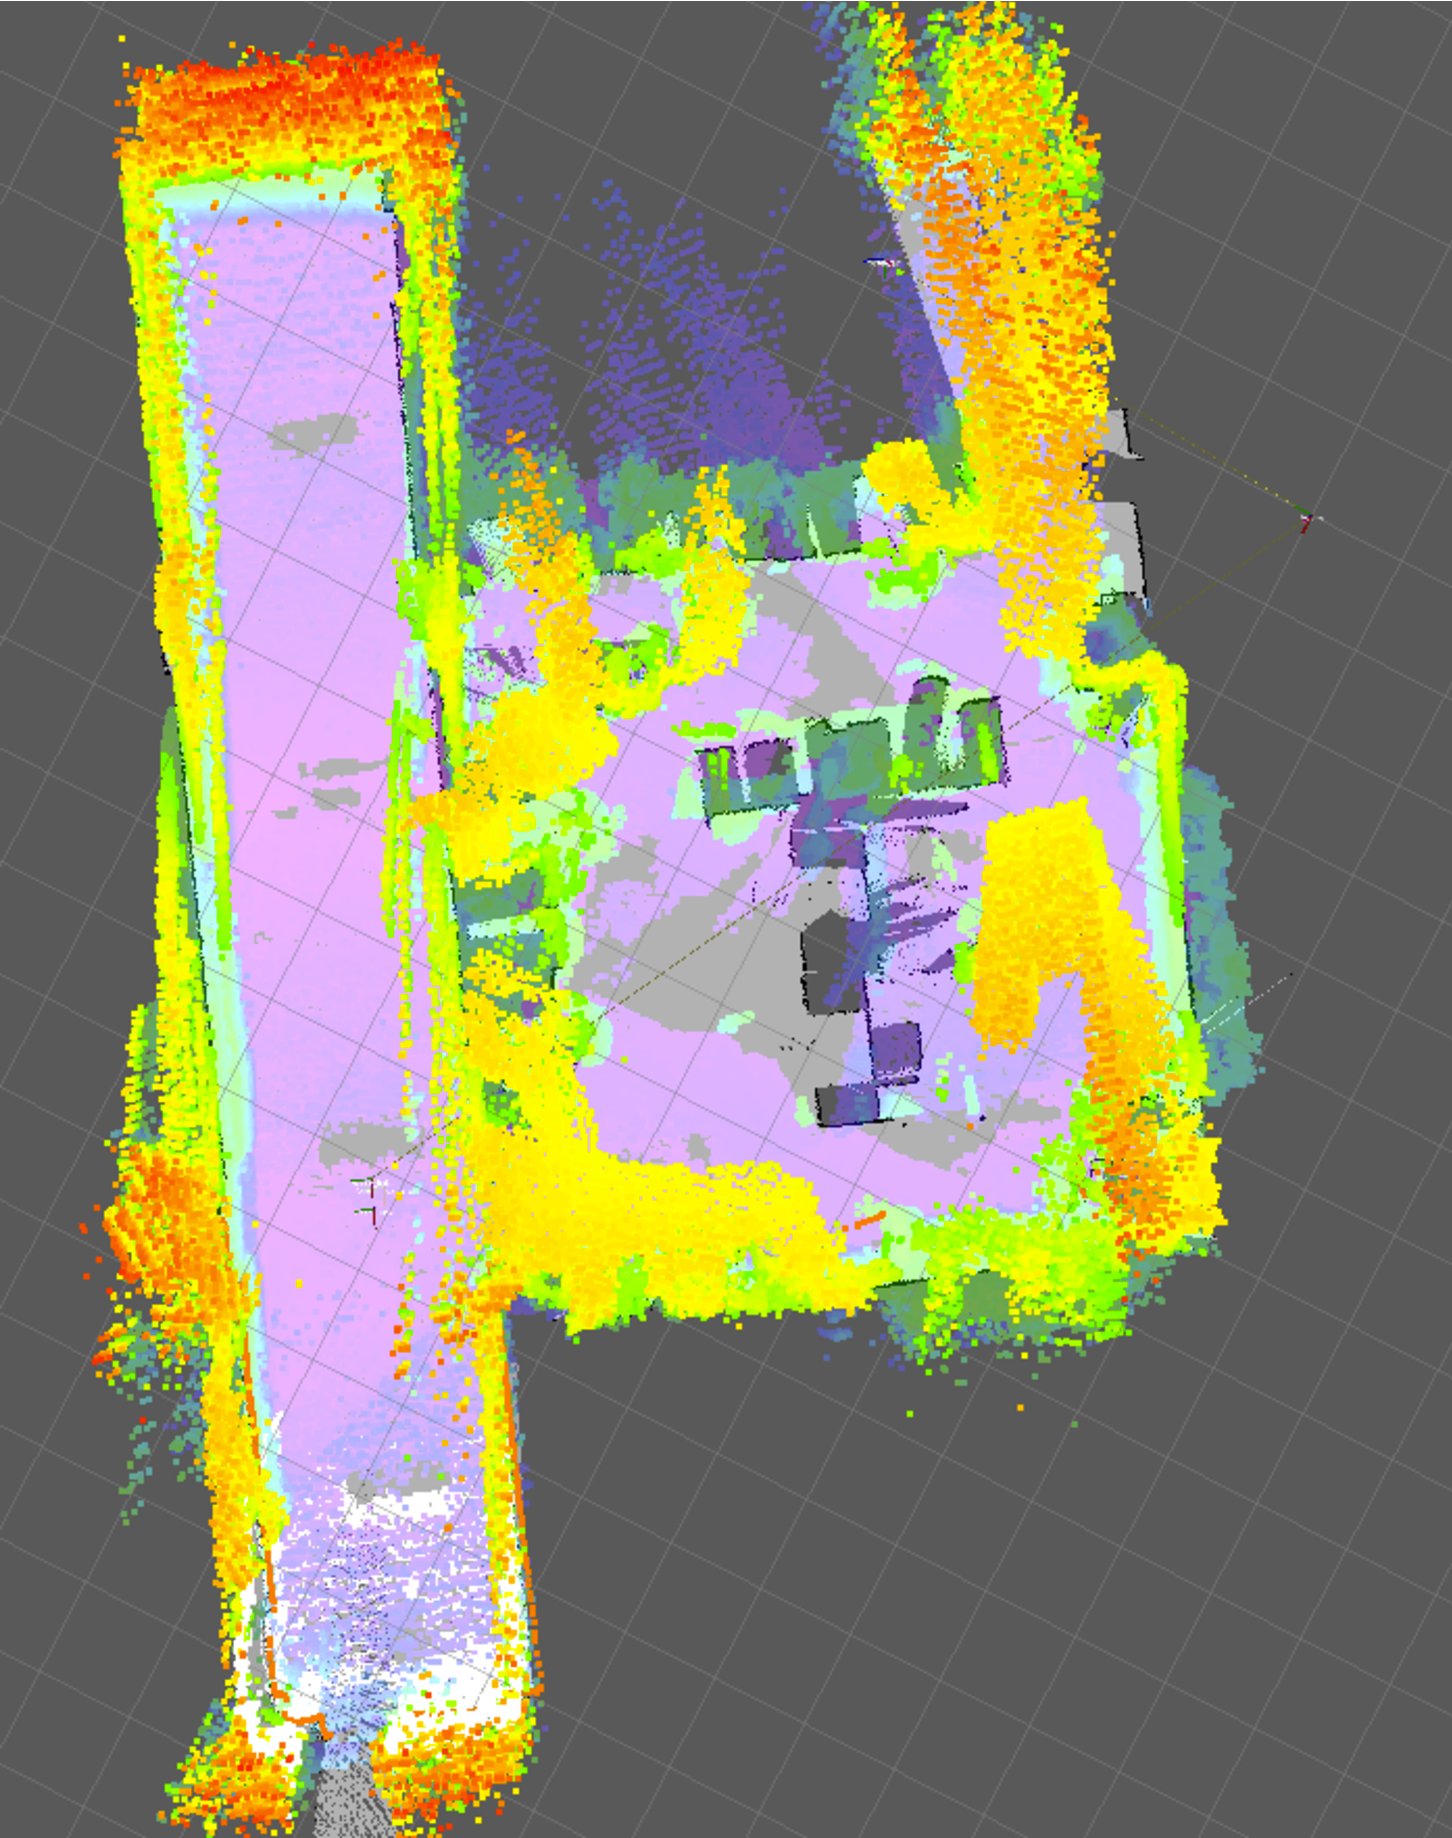
\includegraphics[width=4in,keepaspectratio]{slamvsoctree.pdf}
  \caption{A top down, orthographic view of a three dimensional map generated from Kinect data with a map created by the SLAM library}
  \label{fig:slamvsoctree}
\end{figure}

\subsection{Vehicle Pose Uncertainty}
A major component of the error introduced in mapping with this system is the vehicle pose uncertainty.  In the proposed system, but generally in any system, you have an estimate of your position and orientation, which is generally a combination of multiple sensors or observations and therefore you will often have a grow-bound cycle in the pose estimate uncertainty.  In the proposed system this occurs when a SLAM update occurs.  The SLAM algorithm provides updates to the pose of the vehicle at about 1 Hz, so between these updates the integrated wheel odometry is used to provide poses.  The integrated wheel odometry quickly diverges from the true path of the vehicle and the uncertainty grows quickly, especially when turning in place where the non-linear effects of slip are ignored in the integration of the encoders.  Therefore the uncertainty grows and then is sharply snapped back on a SLAM update.  This effect can be seen in Figure~\ref{fig:uncertainty}, where the mis alignment of the laser data and the map becomes obvious, and then after a SLAM update the pose estimate is much better.  This behavior presents a problem in the mapping, by inserting a point cloud just before the SLAM update the point cloud transform into the map frame is going to be at its worst.

\begin{figure}[ht]
  \centering
  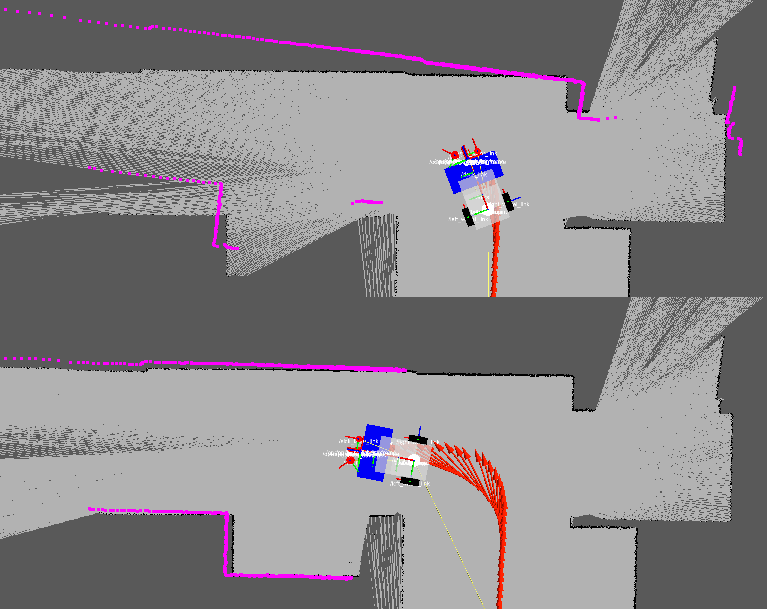
\includegraphics[width=6in,keepaspectratio]{uncertainty.png}
  \caption{This figure shows how the integrated wheel odometry diverges from the pose provided by SLAM when turning.}
  \label{fig:uncertainty}
\end{figure}

Another problem that comes up in the mapping process is that inserting point clouds into the octree map is expensive computationally.  The computation required is affected by the density of the point cloud data and the resolution of the map.  Some sensors, like the Kinect and Xtion Pro Live, produce this point cloud data at high rates, which are as high as thirty hertz.  Due to the computational limitations and the high rate of speed of the data, many of the point clouds have to be dropped.  This is not necessarily a problem for mapping in the system presented here, because the at the speed of the robotic vehicle, 1-2 meters per second, much of the point cloud data is redundant.

A practical solution to both of these problems is to opportunistically select point clouds to insert.  In this system only point clouds that closely proceed SLAM updates are inserted.  It goes without saying that timing is critical here, it is important to match SLAM transform timestamps to point cloud timestamps as closely as possible to avoid further misalignment in the map.

Another solution to this problem is to simply produce a better navigation solution.  Though not pursued in this work, combining the odometry with and IMU or simply a yaw rate gyro with a Kalman Filter would likely reduce the error from the grow-bound cycle in the mapping process.  Point clouds would still need to be throttled, but which were used in the mapping could become arbitrary.

\subsection{Sensor Random Error}
Another, less prominent source of error is the random error in RGBD cameras like the Kinect and the Xtion Pro Live.  There are three sources of error in the this data, loss of precision on depth measurements at greater distances, discretization error on depth measurements, and decreased density of data at greater distances.  The most prominent of these error sources is the variance in the depth measurement.  Khoshelham, K. showed that the random error in the depth of the Kinect data could be modeled from the theoretical principal of the depth sensor\cite{khoshelham2011accuracy}.  In the paper by Khoshelham, K., they show theoretically and experimentally that the depth variance at 4 meters is about 5 centimeters.  This variance changes over distance, with smaller distances yielding more precise measurements than at greater distances.

\begin{figure}[ht]
  \centering
  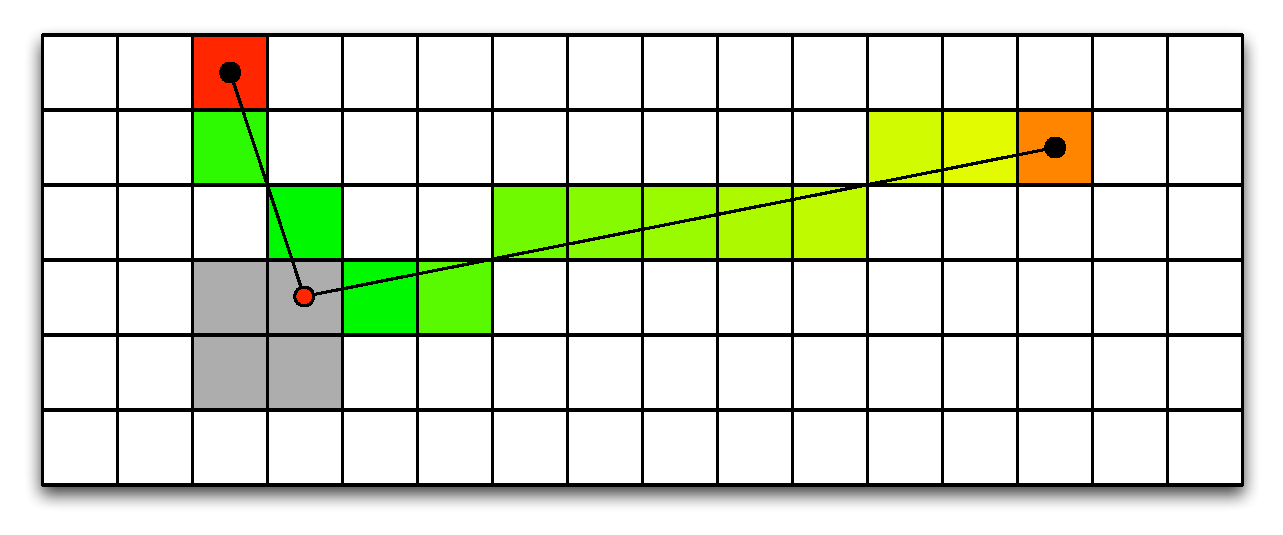
\includegraphics[width=6in,keepaspectratio]{variable_hit_miss.pdf}
  \caption{This figure demonstrates the variable hit and miss values used during ray tracing.}
  \label{fig:variable_hit_miss}
\end{figure}

In order to help minimize this error, a practical solution might be to ignore data that is further than 3 or 4 meters as the variance grows quite large.  Instead this system make a small modification to the method of insertion used by octomap.  Instead of having a constant hit and miss value for ray tracing each point in each point cloud, the hit and miss values change based on the distance to the origin of the sensor.  In this way data that is further from the sensor, especially greater than 3 or 4 meters, is less likely to make a voxel occupied, and less likely to clear an occupied voxel.  This allows the system to incorporate data past 4 meters, but also takes into account the decreased precision.

Figure \ref{fig:variable_hit_miss} shows the effect of long and short ray casts with the above proposed changes.  In the figure the values are varied linearly by distance from the sensor origin, but in practice the system uses a quadratic scaling of the hit and miss values.  Additionally, the scaling does not start until 3 meters from the sensor.  These two changes from the simple linear scaling method reflect the fact that the data under 4 meters is quite good, and the data degrades non-linearly at greater distances.  The results of this tactic on mapping are noticeable in specific situations, but overall improvements are marginal compared to the mapping error induced by errors in the navigation solution.

%%%%%%%%%%%%%%%%%%%%%%%%%%%%%%%%%%%%%%%
%% Chapter: Teleoperation
%%%%%%%%%%%%%%%%%%%%%%%%%%%%%%%%%%%%%%%

\chapter{Teleoperation}\label{chap:teleoperation}
While the three dimensional map is being continuously generated, the client needs to be updated regularly so that the teleoperator has up-to-date telemetry from which to make decisions about the commands to send to the robotic vehicle. This is where the application of the three dimensional mapping to teleoperation occurs. Periodically the probability octree that represents the current best guess as to the occupancy of the environment is converted to a maximum likelihood tree.  This maximum likelihood tree is compared to the client's map of the environment.  The differences are what needs to be sent over the wire to the client.  The differences are sent to the client where the differences are united with the current client map, effectively updating the map used for visualization.  Iterating these actions in parallel with the three dimensional mapping process allows for timely updates and a gracefully degrading difference model based on available bandwidth.

\section{Maximum Likelihood Representation}
The point clouds are initially inserted into an occupancy probability octree where the leafs contain the probability of occupation, but this representation is large and not suited for processing and transmitting the map over the wire in a low bandwidth and/or latent network. The map is therefore periodically transformed into a maximum likelihood version of the probabilistic octree. This transformation is performed by applying a probability high pass filter on the probabilistic octree, where the voxels that are most likely occupied are seen in the transformed octree. The maximum likelihood octree is much more compact because each leaf can be represented with exactly two bits each\cite{octomap}.  Two bits per leaf allows for four unique states for each leaf, of which three are utilized, occupied, unoccupied, or unknown.

\section{Map Streaming}
Once the map is in the maximum likelihood tree format, the map needs to be transmitted to the client. It is possible, however, that there is more data to send than there is bandwidth available. In this case a lower resolution version of the map differences can be sent and more detailed differences can be sent in the future when more bandwidth is available.

\subsection{Octree Set Difference}
The first step in synchronizing the server and client octrees is to figure out what has changed since the last update. In order to determine this the client octree is set differenced with the server octree which should yield the changes in the server from a previous point in time. In order to find the set difference between the two octrees Algorithm \ref{alg:octree_diff} is used. This algorithm is a simple element wise difference and can be thought of as a volumetric difference.

\begin{algorithm}
\caption{Algorithm for Pairwise Difference of Octrees}
\label{alg:octree_diff}
\begin{algorithmic}
  \STATE \COMMENT {$O_0$ is the server occupancy tree}
  \STATE \COMMENT {$O_1$ is the client occupancy tree}
  \STATE \COMMENT {$d$ is the set difference}
  \FORALL{leafs in $O_0$}
    \IF {leaf not in $O_1$}
      \STATE $d\gets leaf$
    \ENDIF
  \ENDFOR
  \RETURN $d$
\end{algorithmic}
\end{algorithm}

\subsection{Bandwidth Adjustment Algorithm}
Once the differences have been determined the differences need to be sent over the network to the client computer to be united with the current client map. In the case that there is not enough available bandwidth the differences can be reduced by differencing the two octrees at a lower resolution. The lower resolution versions of the trees can be obtained by limiting the depth of the query into the octree. If the leaf size of the octree is 2 centimeters, then reducing the query depth by one will result in a subtree with leafs of size 4 centimeter, this phenomenon is demonstrated in a map of the Shelby Center at Auburn University by Figure \ref{fig:treedepth}.  The visualization in Figure \ref{fig:treedepth} was done using octovis\cite{octomap}, which is part of octomap.

\begin{figure}[ht]
  \centering
  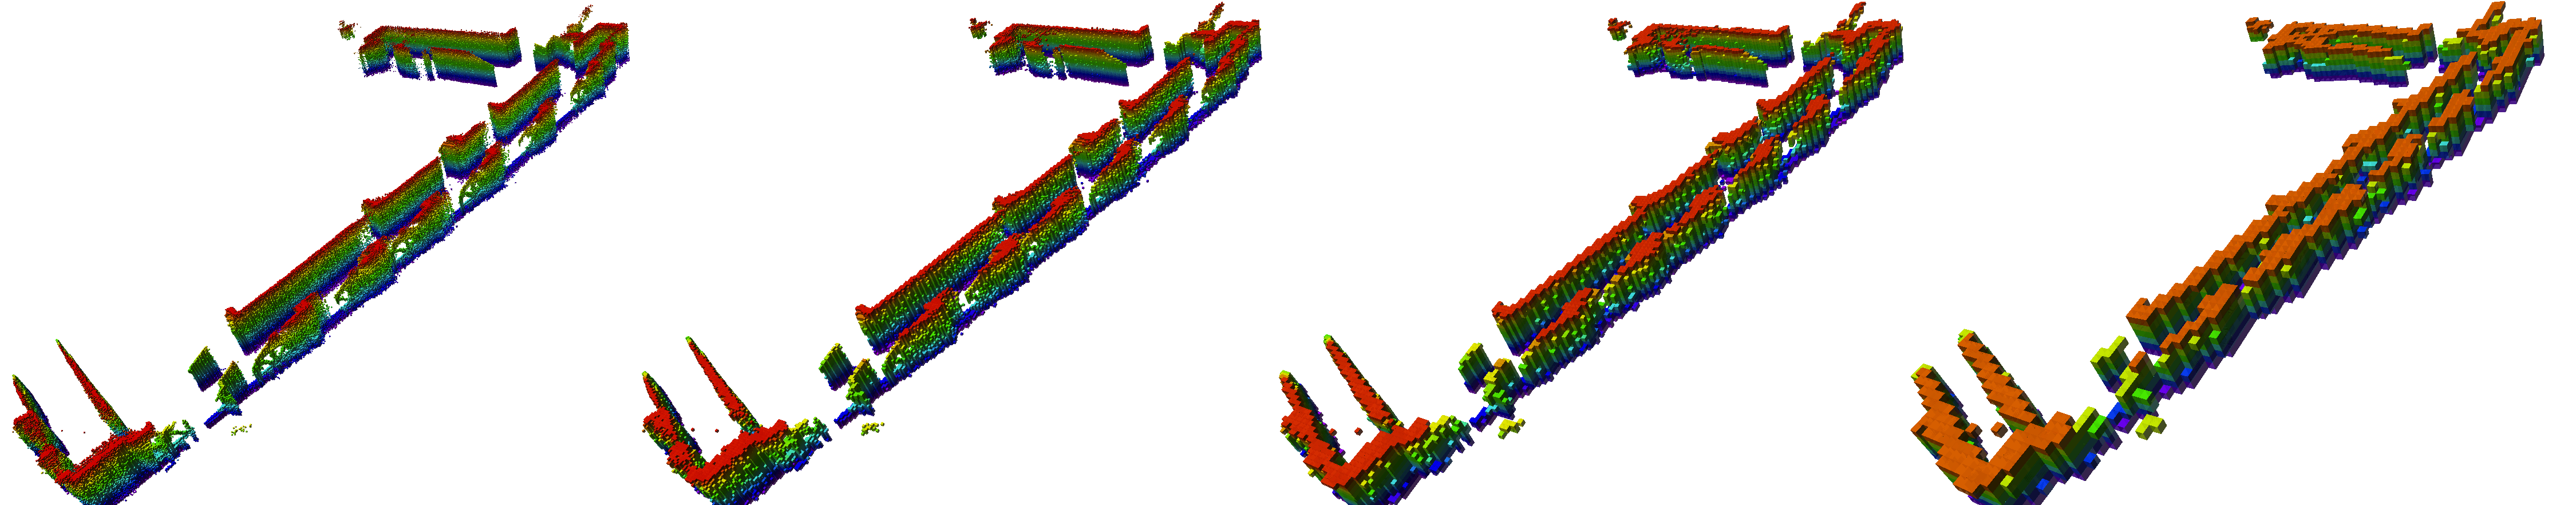
\includegraphics[width=6.5in,keepaspectratio]{ShelbySE_2f_combined_octovis.png}
  \caption{Partial map of a hallway showing the effect of limiting the query 
           depth.  From left to right the resolution is 0.05m, 0.1m, 0.2m,
           and 0.4m.}
  \label{fig:treedepth}
\end{figure}

The algorithm for selecting the depth is proposed in Algorithm \ref{alg:bandwidth} and simply continues to degrade the resolution until there is enough bandwidth to transmit or until there resolution cannot be degraded further.

\begin{algorithm}
\caption{Algorithm for Determining Difference Depth}
\label{alg:bandwidth}
\begin{algorithmic}
  \STATE \COMMENT {$O_0$ is the server map octree}
  \STATE \COMMENT {$O_1$ is the client map octree}
  \STATE \COMMENT {$d$ is the set difference}
  \STATE \COMMENT {$B_d$ is the bandwidth required to transmit the diff}
  \STATE \COMMENT {$B_a$ is the available bandwidth}
  \STATE \COMMENT {$T_u$ is the update period in seconds}
  \STATE \COMMENT {$h_{max}$ is the maximum size of a leaf to be transmitted}
  \STATE $i\gets 0$
  \REPEAT
    \STATE $O_0 \prime = depth(O_0,height(O_0)-i)$
    \STATE $O_1 \prime = depth(O_1,height(O_1)-i)$
    \STATE $d = O_0 \prime \bigcup O_1 \prime $
    \STATE $B_d = size(d) / T_u$
    \STATE $B_a = currentAvailableBandwidth()$
    \STATE $i = i + 1$
  \UNTIL {$B_d\le B_a \| resolution(i) \ge h_{max}$}
  \RETURN $d$
\end{algorithmic}
\end{algorithm}

The depth function simply returns a subtree of the given tree at the height given, and the height function gives the height of the tree specified.  The resolution function simply returns the dimension of a leaf at the given level.  The current available bandwidth function could be implemented in several ways, but the topic of available bandwidth estimation has been covered in the literature.\cite{prasad2003bandwidth} The principal behind the bandwidth estimation is looking at metrics like round-trip-time, average delay, packet loss, and throughput to determine the bandwidth currently available.  During testing the bandwidth will be artificially controlled to exercise this component of the system.  Artificially controlling the bandwidth used by the mapping system will also allow for quality of service to be enforced on it.  This would allow the system to prioritize things like teleoperation commands, video, or other telemetry over the map update.

\subsection{Octree Set Union}
The final stage of synchronizing the server and client octrees is to unite the differences with the client octree. This is just a simple union operation and can be performed by simply inserting every voxel of the differences into the client map using the normal octree insertion method.\cite{meagher1982geometric}

\section{Visualization}
Talk about the map visualization.

\section{Teleoperator Input}
Talk about the interface for the teleoperator to control the vehicle.

%%%%%%%%%%%%%%%%%%%%%%%%%%%%%%%%%%%%%%%
%% Chapter: Latency Reduction
%%%%%%%%%%%%%%%%%%%%%%%%%%%%%%%%%%%%%%%

\chapter{Latency Reduction}\label{chap:latency_reduction}
This chapter talks about latency reduction techniques and their implementation.

\section{Vehicle Model}
Talk about the kinematic vehicle model.

\section{Interface}
How is the model used to help the teleoperator?

%%%%%%%%%%%%%%%%%%%%%%%%%%%%%%%%%%%%%%%
%% Chapter: Experiments
%%%%%%%%%%%%%%%%%%%%%%%%%%%%%%%%%%%%%%%

\chapter{Experiments}\label{chap:experiments}
This chapter outlines the experiment goals, setup, and results.

\section{Experiment Goals}
Talk about what we hope to achieve by including a real system.

\section{Experimental Setup}\label{sec:experimental_setup}
Talk about the myriad systems used to talk data and their capabilities, etc...

\section{Experimental Results}
Pretty pictures and teleoperation analysis, also latency stats.

%%%%%%%%%%%%%%%%%%%%%%%%%%%%%%%%%%%%%%%
%% Chapter: Conclusions
%%%%%%%%%%%%%%%%%%%%%%%%%%%%%%%%%%%%%%%

\chapter{Conclusion}\label{chap:conclusion}
This chapter draws some conclusions and looks to future work.

\section{Future Work}
Some thing about future work.

\subsection{Improved Mapping}
Talk about KinectFusion again.

\subsection{Dynamic Vehicle Models}
Talk about how a dynamic vehicle model might improve the latency reduction system.

\subsection{More Latency Reduction Studies}
More data is required to properly quantify the latency reduction system's effectiveness.  (Likely)

%=================
%=================
%======fin========
%=================
%=================

%If you do not need the List of Abbreviations\nomenclature{LoA}{List of Abbreviations}, comment the nomencl package and associated nomenclature commands. 


%%%%%%%%Two options for having a bibliography. If you use a separate file or multiple files:

%%%%% where the files are robotics.bib, imageprocessing.bib and/or thesis.bib. 
\bibliographystyle{IEEEtran}
\bibliography{references}
%Or you can include the bibliography entries directly:

\appendix
\chapter*{Appendices\addcontentsline{toc}{chapter}{Appendices}}
\chapter{Some C++ Source Code}
\begin{singlespace}
\begin{verbatim}
#include <iostream>

using std::cout;
using std::endl;

int main(void) {
  cout << "Hello World." << endl;
  return 0;
}
\end{verbatim}
\end{singlespace}

\end{document}

